\section{Methodology}%
\label{sec:method}
%\FloatBarrier

As described in \cref{sec:problem}, the input data comes in the form of a
PDF file which can be converted into plaintext XML data containing lines of text
along with each line's bounding box. There are two systems in play here; the
main system is a convolutional neural network classifier that acts on the XML
data. Further details on this are provided in \cref{sec:sup}. The second
system is the unsupervised preprocessor whichs acts on the PDF data and writes
its output as an additional property into the XML data, which is elaborated upon
in \cref{sec:unsup}. \Cref{fig:overview} shows a high-level
overview of the two systems and how they interact.

\begin{figure}[tb]
  \centering
  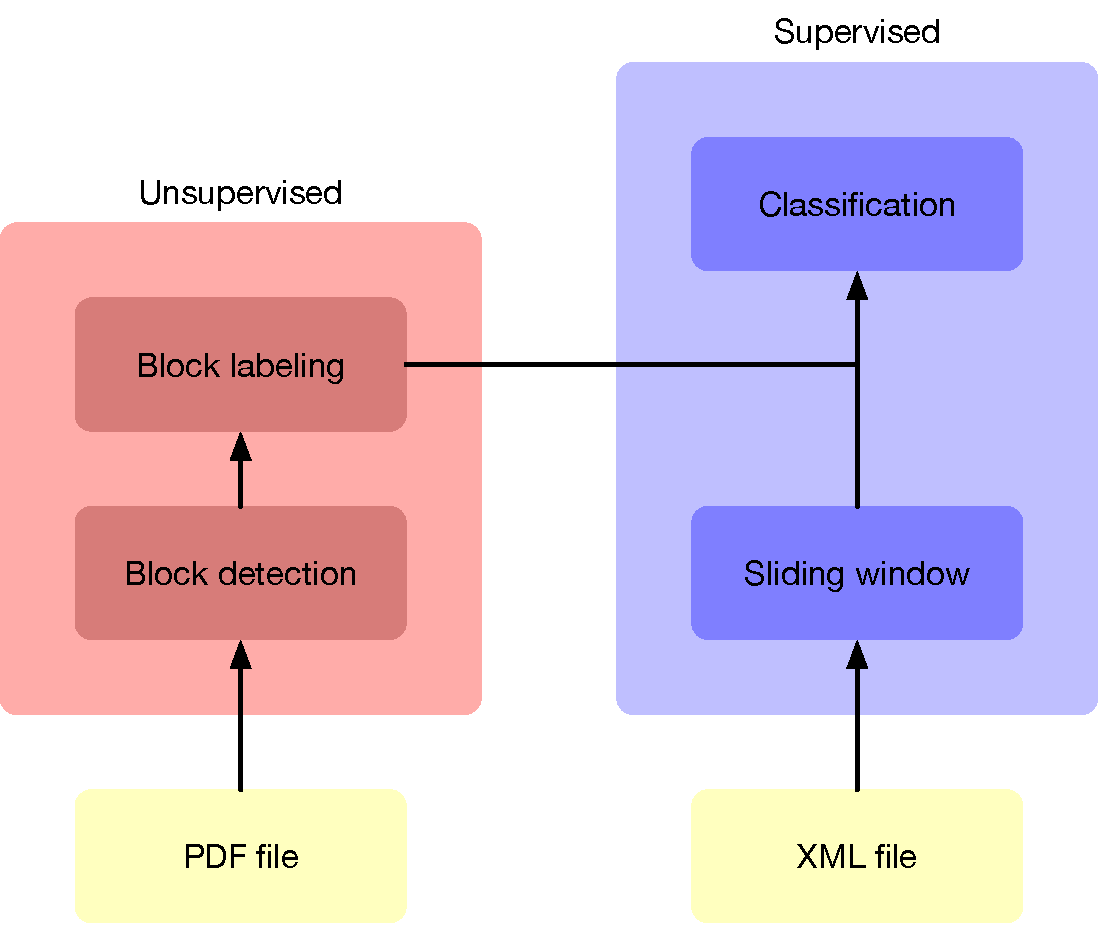
\includegraphics[width=\textwidth]{figures/layout.pdf}
  \caption{A high-level overview of the system. The unsupervised block augments
  the input to the classifier.\label{fig:overview}}
\end{figure}

\subsection{Unsupervised}%
\label{sec:unsup}
The unsupervised algorithm is inteded to detect and classify blocks of text in the
PDF file; \Cref{fig:clustered} shows an example. This approach is based on
work by \textcite{klampfl2014unsupervised}, and consists of two separate
clustering steps. First, individual characters (the fundamental objects
available in a PDF file) are clustered together into blocks of semantically
relevant text. These could be, for example,  paragraphs, section headers or page decoration.
By using the bounding boxes of the blocks, they can be clustered based on their
shape and some additional metadata (e.g.\ occurrence of font types and sizes).
The rest of this section will go into details on the two clustering steps.

\begin{figure}[tb]
  \centering
  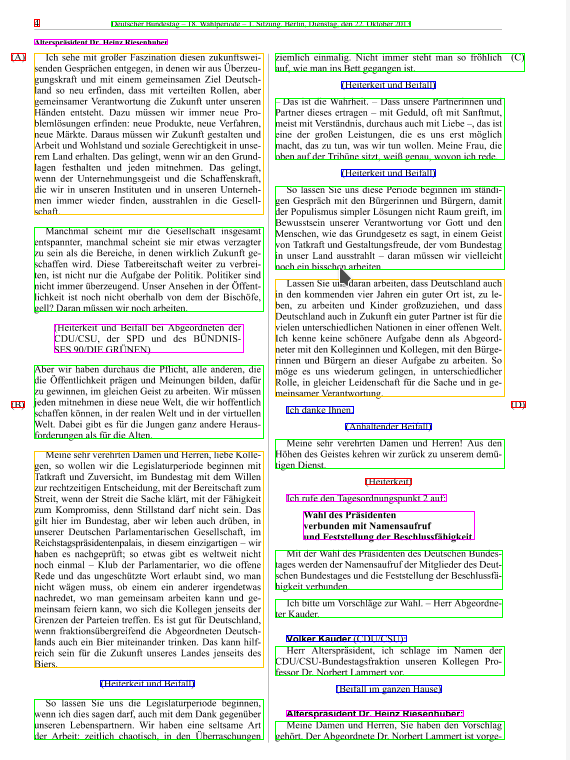
\includegraphics[height=0.5\textheight]{figures/cluster_example.png}
  \caption{An example of clustered blocks of text. Blocks with the same outline
  color belong to the same cluster.\label{fig:clustered}}
\end{figure}

\subsubsection{Hierarchical Agglomerative Clustering}
The first step is performed using hierarchical agglomerative clustering (HAC),
an unsupervised bottom-up clustering algorithm that constructs a hierarchical
tree of clusters (in this context referred to as a \emph{dendrogram}). An
example is shown in \cref{fig:hac}. The algorithm gets fed the individual
characters present in the PDF files, then iteratively groups the two closest
clusters (the initial inputs being regarded as clusters of one element) together
until only a single cluster remains. This process involves two parameters:
\begin{enumerate}
\item The distance function between two characters.
\item The distance function between two clusters of characters.
\end{enumerate}
The first parameter is trivially chosen to be the Euclidian distance between the
coordinates of the two characters. The second parameter is called the
\emph{linkage} and has several common options, the most basic of which are:
\begin{itemize}
\item Single-linkage: The distance between clusters is based on the closest two
  elements: \[ d(A, B) = \min \{ d(a, b) : a \in A, b \in B \} \]
\item Maximum-linkage: The distance between clusters is based on the furthest two
  elements: \[ d(A, B) = \max \{ d(a, b) : a \in A, b \in B \} \]
\item Average-linkage: The distance between clusters is based on the average
  distance of its elements:
  \[ d(A, B) = \frac{1}{|A||B|} \sum_{a \in A}\sum_{b \in B} d(a, b) \]
\end{itemize}
Additionally there are more involved linkage criteria, such as the Ward method
which minimizes the variance within clusters. Although these more complex
methods would generally be favored, in this specific context single-linkage
clusters is actually the best option\citep{klampfl2014unsupervised}. This is due
to its tendency to form long, thin clusters; this mirrors the nature of text, in
particular words and sentences (which are just long, thin strings of letters and
words respectively).
As an additional bonus, it is the most computationally efficient method.
While the general time complexity for HAC is
in $\mathcal{O}(n^3)$, clever algorithms exist for single-linkage clustering
that fall in $\mathcal{O}(n^2)$ \citep{sibson1973slink}, making it far more
usable on larger datasets.

\begin{figure}[tb]
  \centering
  \begin{subfigure}[b]{0.40\textwidth} 
    \centering
    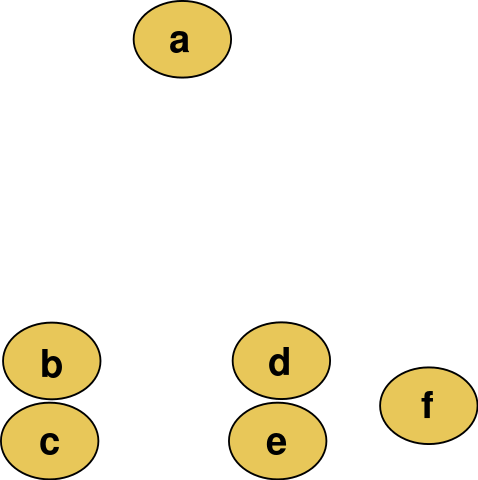
\includegraphics[width=\textwidth]{figures/dendrogram1.png}
    \caption{Before}
  \end{subfigure}
  \hspace{0.10\textwidth}
  \begin{subfigure}[b]{0.40\textwidth}
	\centering
    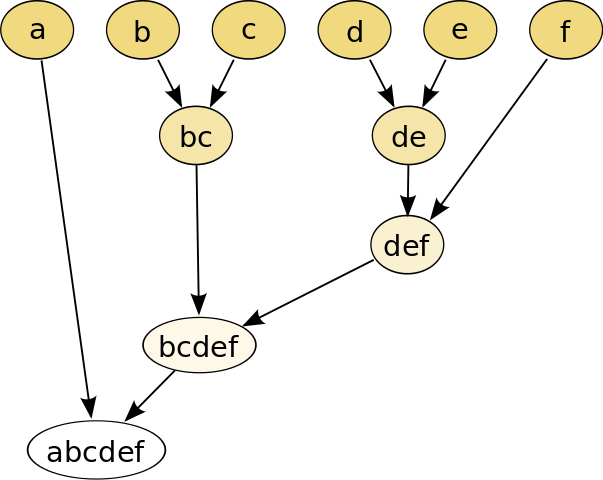
\includegraphics[width=\textwidth]{figures/dendrogram2.png}
    \caption{After}
  \end{subfigure}
  \caption{An example of hierarical agglomerative clustering, where the nodes
  are clustered by distance.\label{fig:hac}}
\end{figure}

After the dendrogram is constructed, it has to be cut at some level to obtain
the desired blocks of text. Clustering can optionally be rerun using the newly
found clusters as basic elements. This way, the document can incrementally be
clustered from characters into words, words into lines, and finally lines into
paragraphs. Both the level at which to cut the tree and the number of times to
recluster are to be manually tuned based on the particular set of documents.

\subsubsection{K-Means}
The extracted blocks from the previous step are then clustered according to
their similarity based on the following metrics:
\begin{itemize}
  \item Width of the cluster
  \item Height of the cluster
  \item The ID of the most common font occurring in the cluster
  \item The size of the most common font occurring in the cluster
\end{itemize}
This is done using K-means clustering, with the value of $k$ being varied for
experimental purposes.

\subsection{Supervised}%
\label{sec:sup}
After the data is augmented by the previously described clustering algorithms,
it's fed into a convolutional neural network for classification. Since the
documents have a dual column layout (meaning each line of text is pretty short)
and classification is based on the lines from the document, a sliding window is
used to supply more context. The text content of this window is then tokenized
(such that words as well as each individual punctuation mark are a token)
and fed into a standard convolutional neural network
architecture\citep{kim2014conv}, with the label (i.e.\ does or does not start a
new speech) being provided by the center element of the window.
First an embedding layer is used to learn a high-dimensional representation of
the tokens (no pre-trained embeddings were used because of both the specialized
political domain of the data as well as a lack of quality pre-trained German
models), followed by a single convolutional layer, consisting of multiple
filters each followed by 1-max pooling (a more in-depth explanation is provided
in \cref{sec:conv}). The output of the filters is then concatenated into a
single feature vector, which is combined with the clustering data in one of two
ways, which will both be evaluated:
\begin{enumerate}
  \item The cluster types of each element in the window are added to the
    feature vector.
  \item An additional smaller LSTM is applied to the cluster types of each
    element in the window, the output of which is concatenated with the feature
    vector.
\end{enumerate}
The resulting feature vector is then fed into a fully-connected neural network.
This network features one hidden layer with a ReLU activation ($\mathrm{relu}(x)
= \max(0, x)$) and a single output node with a sigmoid activation. The layout of
this system is detailed in \cref{fig:model_full} along with its parameters and
their baseline value.

The network is trained for 100 epochs, stopping early once no significant
improvement has been made on a small validation set for 10 epochs in a row. The
optimisation process is done using the Adadelta\citep{adadelta}
algorithm\footnote{Why not Adam\citep{adam}? The architecture\citep{kim2014conv}
and survey paper\citep{zhang2015conv} that this work is based on both date to
roughly the year when the Adam paper was published, and thus likely predate the
widespread acceptance of Adam as a de facto standard. Since a full analysis of
different optimizers is outside the scope of this thesis and some quick informal
tests showed no difference between using Adadelta or Adam, there is no reason to
deviate from the survey.}, with binary cross-entropy as the loss function and
the training data delivered in batches. Regularisation is done through a
combination of dropout\citep{dropout} and an upper limit on the L2 norm of each
weight vector\citep{l2norm}. Further explanations of the optimisation process
and the regularisation methods are provided in \cref{sec:optim} and
\cref{sec:reg} respectively.

\begin{figure}[p]
  \centering
  \begin{subfigure}[b]{0.45\textwidth}
    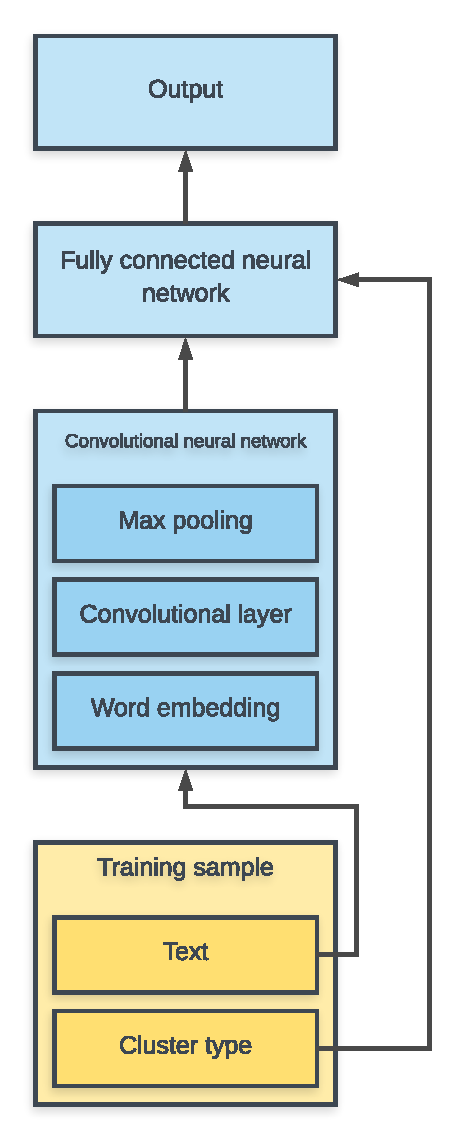
\includegraphics[width=\textwidth]{figures/nn_layout.pdf}
    \caption{The layout of the supervised portion of the system. The input data
      contains text and a cluster type assigned by the unsupervised portion. The
      text gets put into a convolutional neural network, the output of which is
      fed together with the cluster type into a fully connected neural network.
      The sigmoid function is applied to the output of this final neural network
    to obtain the classification.\label{fig:nn_layout}}
  \end{subfigure}
  \hspace{0.05\textwidth}
  \begin{subfigure}[b]{0.45\textwidth}
    \begin{subfigure}[b]{\textwidth}
      \centering
      \begin{tabular}{lr}
	\toprule
	Parameter & Default value \\
	\midrule
	Window size & 9 \\
	Word embedding size & 300 \\
	Number of filters & 100 \\
	Filter sizes & 4, 5, 6 \\
	Activation & ReLU \\
	Pooling type & 1-max \\
	\bottomrule
      \end{tabular}
      \caption{The default parameters used in the convolutional neural network.}
      \vspace{1cm}
    \end{subfigure}

    \begin{subfigure}[b]{\textwidth}
      \centering
      \begin{tabular}{lr}
	\toprule
	Parameter & Default value \\
	\midrule
	Number of hidden layers & 1 \\
	Hidden layer size & 50 \\
	Hidden layer activation & ReLU \\
	Number of outputs & 1 \\
	Output activation & Sigmoid \\
	\bottomrule
      \end{tabular}
      \caption{The default parameters used in the fully-connected neural network.}
      \vspace{1cm}
    \end{subfigure}

    \begin{subfigure}[b]{\textwidth}
      \centering
      \begin{tabular}{lr}
	\toprule
	Parameter & Default value \\
	\midrule
	Batch size & 50 \\
	Dropout rate & 0.5 \\
	Learning rate & 1.0 \\
	$\rho$ & 0.9 \\
	Maximum L2 norm & 3 \\
	\bottomrule
      \end{tabular}
      \caption{The default parameters used for the optimisation
	process.\label{tbl:params}}
    \end{subfigure}
  \end{subfigure}
  \caption{The model and its parameters.\label{fig:model_full}}
\end{figure}

\subsubsection{Optimisation process}\label{sec:optim}
Optimisation is done using the Adadelta update rule\citep{adadelta}. This is
easiest to explain by starting with the basic mini-batch stochastic gradient
descent algorithm (SGD). At each iteration $t$, the network parameters $\theta$
are updated based on some calculation:
\begin{equation}
  \theta_{t+1} = \theta_{t} - \Delta\theta_t
\end{equation}
The difference between optimization algorithms is how $\Delta\theta$ is
calculated. With SGD, it is simply
\begin{equation}
  \Delta\theta_t = \mu \loss{t}
\end{equation}
where $\mathcal{L}$ is the loss function (in this case, the binary cross entropy
between the predicted labels and the true labels), and $\mu$ is an arbitrary
learning rate between 0 and 1. This learning rate is a tricky parameter to set;
too low and learning will take ages, too high and the network will fail to
converge because the steps taken are too big. One way to improve this is by
using the Adagrad\citep{adagrad} algorithm. While SGD uses a single learning
rate for the entire parameter vector, Adagrad (which stands for ``adaptive
gradient'') adapts the learning rate for each individual parameter; frequently
updated parameters get a lower learning rate, while less frequently updated
parameters are updated with a higher learning rate. This is done by simply
dividing the learning rate with the L2 norm of the sum of all previous gradients:
\begin{gather}
  g_{t} = \loss{t} \\
  \Delta\theta_t = \frac{\mu}{\sqrt{\sum^{t}_{\mathcal{T}=1}g_{\mathcal{T}}^2}} g_{t}
\end{gather}
This has been found to work very well, in particular in natural language
processing and computer vision where features are often sparse, but it has two
drawbacks:
\begin{enumerate}
  \item A suitable value for the global learning rate $\mu$ has to be
    manually provided.
  \item Since the learning rate is rescaled using a monotonically increasing sum of
    previous gradient magnitudes, the learning rate will converge to zero.
\end{enumerate}
Adadelta nullifies these drawbacks by eliminating the global learning rate and
restricting the accumulation of gradients to a window of recent updates. First
of all, the sum over all previous gradients is replaced by an exponentially
decaying average of the squared gradients, referred to as $E[g^2]$:
\begin{equation}\label{eq:rms}
  E[g^2]_t = \rho E[g^2]_{t-1} + (1 - \rho) g_t^2
\end{equation}
Here $\rho$ is a constant representing the rate of decay; this decaying sum
serves as a more efficient approximation of an actual window of past gradients,
which would require far more memory to store (considering both the huge number
of parameters in a neural network and the memory constraints of running on a GPU).
Substituting this into the Adagrad algorithm gives us:
\begin{align}
  \Delta\theta_t &= \frac{\mu}{\sqrt{E[g^2]_t}} g_{t} \\
		 &= \frac{\mu}{RMS[g]_t} g_{t}
\end{align}
The quantity $\sqrt{E[g^2]_t}$ is called the \emph{root mean square} of $g$,
which occurs often enough in optimisation algorithms that it is often
abbreviated as $RMS[g]$. As a final step, the learning rate $\mu$ is eliminated
by replacing it with a decaying average of the previous gradient updates,
similar to \cref{eq:rms}.
\begin{equation}
  \Delta\theta_t = \frac{RMS[\theta]_{t-1}}{RMS[g]_t} g_{t}
\end{equation}

\subsubsection{Regularisation}\label{sec:reg}
Dropout\citep{dropout} is a Regularisation method that is rather crude at first
glance; on each batch update, each node in the neural network has a probability
$p$ of outputting zero (i.e.\ the node being ``disabled''). As a result, nodes
cannot rely on the output of any other node being present, preventing
co-adaptation and as a result reducing the probability of overfitting on the
training data. Dropout is only active during training; when running the network
in evaluation mode, all nodes are active and the outputs are rescaled by a
factor of $1 - p$ to account for the now higher activation values.
There is another way to view dropout. It is commonly known that neural network
(or really any machine learning classifier) performance can be improved by
training a large number of them and averaging their outputs. Since every
combination of nodes disabled by dropout could be considered a unique neural
network, dropout acts as computationally cheap approximation to averaging
multiple networks.

In addition to dropout, a maximum L2 norm is imposed on each node's incoming
weight vector. If the weight vector's L2 norm exceeds this limit, it is rescaled
so that its new norm is equal to the maximum allowed norm; otherwise the weight
vector is left alone:
\begin{equation}
  \label{eq:norm}
  \vect{w} = \begin{cases}
    \vect{w}\,                          & \text{if } ||\vect{w}||^2 \leq n \\
    n \frac{\vect{w}}{||\vect{w}||^2} & \text{otherwise}
  \end{cases}
\end{equation}
This differs from the more common L2-regularisation --- where the combined L2
norm of all weight vectors is added to the loss function --- in that the weights
are not being continuously pushed towards zero, making it a milder form of
regularisation that allows for a bit more complexity in the model.

\subsubsection{Convolutional Neural Networks}\label{sec:conv}
In addition to explaining how a convolutional neural network works, this section
will additionally go into why the choice was made to use a convolution neural
network, rather than a recurrent neural network (which is more strongly
associated with text processing) or any other machine learning algorithm.
Starting with the basics, text is inherently troublesome because it produces
3-dimensional data: there is a feature vector for each word, and some (either
variable or predetermined through padding) amount of words per text. This makes
each training sample a 2-dimensional matrix, which then gets stacked in the
depth dimension to produce 3-dimensional training data. This clashes with the
tendency of usual machine learning algorithms to work on 2-dimensional data,
assuming a feature vector for each sample rather than a matrix. There are three
common methods to deal with this:
\begin{itemize}
\item Bag of words
\item Convolutional neural networks
\item Recurrent neural networks
\end{itemize}

Aside from being completely different methods, they differ in a major way in how
they handle the sequential nature of text (i.e.\ the words in a sentence have a
meaningful order). The bag of words approach is the
simplest in that it simply disregards this sequential nature entirely, instead creating
what is essentially a histogram of word occurrences. This downsamples each
sample from a feature matrix to a feature vector, allowing the use of
conventional machine learning algorithms (most commonly support vector
machines). While the sequential information can be kept to some degree by using
histograms of $n$-grams rather than words (unigrams), this causes the size of
the input data to scale exponentially with the value of $n$.

Convolutional neural networks (CNNs) work by taking a number of filters
(sometimes called kernels or feature maps) of a specified size and convolving
these over the input data. A simplified example using one filter is shown in
\cref{fig:cnn}.
\begin{figure}[tb]
  \centering
  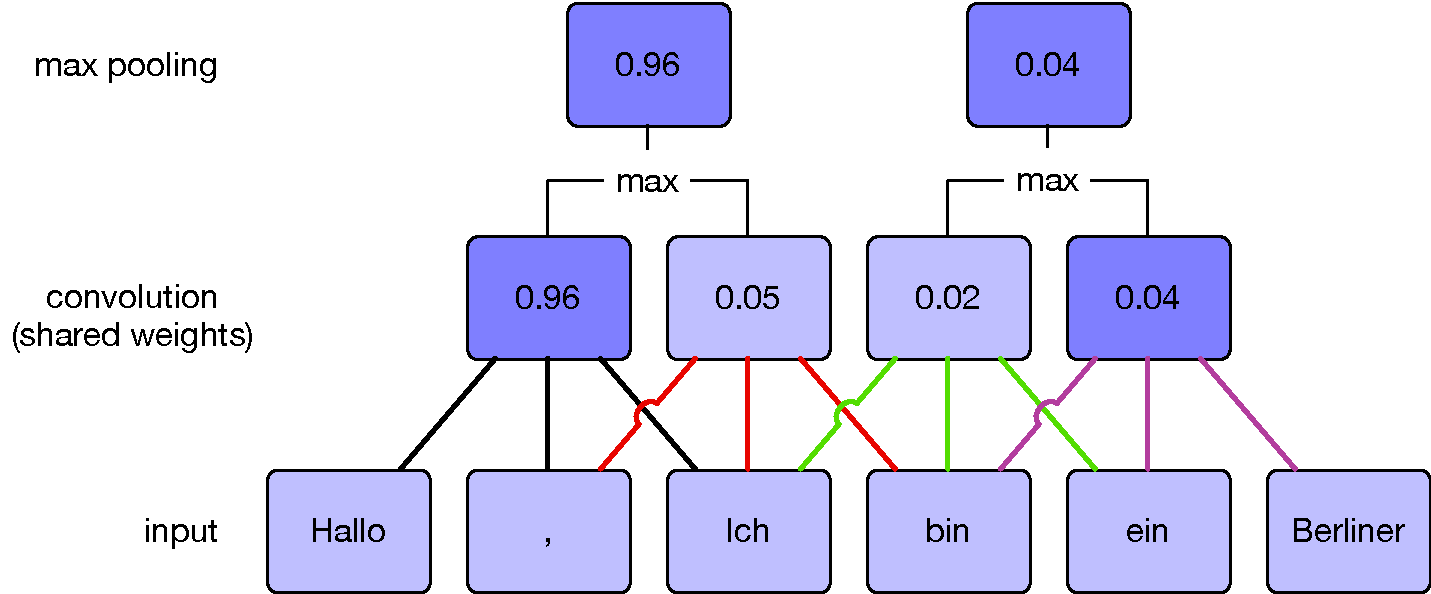
\includegraphics[width=\textwidth]{figures/cnn.pdf}
  \caption{A simplified convolutional neural network with one filter and
  max pooling.\label{fig:cnn}}
\end{figure}
In this example, the input text is convolved with a filter with a width of 3 and
a stride of 1 --- that is, each application of the filter considers three
subsequent input elements, after which the window is shifted one space to the
right. This filter is essentially a small neural network mapping three items to
one output value, whose weights are reused for each application of the filter.
Reusing the weights in this way (weight sharing) prevents the number of
parameters in the network from spiraling out of control.
\citep{lecun1995convolutional} After the application of this convolution layer,
the responses of the filter form a new sequence of roughly the same size as the
input (minus a few due to missing the edges). The next step is to downsample
this sequence by means of a \emph{max pooling} layer, which maps all values
within a window to the maximum value amongst those values. While conceptually
similar to a convolution, this step generally does not involve overlap, instead
either setting the stride to the same value as the window size (usually 2) or
reducing the entire sequence to 1 value (1-max pooling). The reason for this is
twofold:
\begin{enumerate}
\item It downsamples the data, reducing the amount of parameters
  required further on in the network.
\item It adds translation invariance to the feature detected by this filter. The
  example filter of \cref{fig:cnn} reacts strongly to the
  first three words. Without the pooling layer, changing the
  location of these words in the input would similarly change the
  location of the high activation in the intermediate representation; this would
  be translation \emph{equivariance}. The more aggressively the pooling is
  applied, the higher the degree of invariance (with full translational
  invariance being achieved with 1-max pooling).
\end{enumerate}
This combination of convolution followed by pooling can be repeated multiple
times as desired or until there is only a single value left as output from the
filter. Finally, the outputs of all filters are concatenated and fed into a
regular neural network.

While CNN architectures in computer vision are generally very deep, they tend to
be very shallow in natural language processing; commonly just a single
convolution followed by 1-max pooling \citep{zhang2015conv}. 

\subsubsection{Difference between convolutional and recurrent neural networks}
Recurrent neural networks (in particular LSTMs or GRUs) are seemingly the most
natural fit for language processing, since they process an entire sequence and
are therefore fully conditioned on the word order (as opposed to the
convolutional neural networks which tend to learn translation invariant ngram
features). In spite of this, the decision to use convolutional neural networks 
is based on two factors:
\begin{enumerate}
\item In practise, the performance for classification tasks does not differ
  between the convolutional and recurrent neural networks.\citep{cnnrnn}
\item The computations in convolutional networks are highly independent of
  each other, allowing for great parallelization (in particular with regards to
  running on a GPU). In contrast, LSTMs are bottlenecked by the fact that each
  calculation is dependent on the previous calculations. As a result, CNNs
  achieve far higher training speeds.\citep{facebook}
\end{enumerate}

%%% Local Variables:
%%% mode: latex
%%% TeX-master: "report"
%%% End:
